\documentclass[conference]{IEEEtran}
\IEEEoverridecommandlockouts
% The preceding line is only needed to identify funding in the first footnote. If that is unneeded, please comment it out.
\usepackage{cite}
\usepackage{amsmath,amssymb,amsfonts}
\usepackage{algorithmic}
\usepackage{textcomp}
\usepackage{xcolor}
\usepackage{circuitikz}
\usetikzlibrary{arrows.meta,positioning,calc,fit}
\usepackage{silence}
\usepackage{amsthm}
\usepackage{enumitem}
\usepackage{eufrak}
\usepackage{tabularx}
\usepackage{lipsum}
\usepackage{pifont}
\usepackage{yfonts}
\usepackage{booktabs}
\usepackage{float}
\usepackage{amsmath}
\usepackage{amssymb}
\usepackage{comment}
\usepackage{amsfonts}
\usepackage{csquotes}
\usepackage{fancyhdr}
\usepackage{graphicx}
\usepackage{listings}
\usepackage{mathrsfs}
\usepackage{setspace}
\usepackage{textcomp}
\usepackage{multicol}
\usepackage{blindtext}
\usepackage{enumerate}
\usepackage{kantlipsum}
\usepackage[hidelinks]{hyperref}
\def\BibTeX{{\rm B\kern-.05em{\sc i\kern-.025em b}\kern-.08em
    T\kern-.1667em\lower.7ex\hbox{E}\kern-.125emX}}
\renewcommand{\refname}{Referencias}
\renewcommand{\lstlistingname}{Listado}
% Marcador de contenido pendiente (se muestra en rojo).
\newcommand{\PEND}[1]{{\color{red}[#1]}}
\begin{document}

\title{Informe final de una microrred DC de 48 V emulada: condiciones nominales y ante perturbaciones sobre STM32 y ESP32\\
}

\author{\IEEEauthorblockN{Sofía Parra Rozo}
\IEEEauthorblockA{\textit{Departamento de Ingeniería Eléctrica y Electrónica} \\
\textit{Universidad de los Andes}\\
Bogotá, Colombia \\
s.parrar2@uniandes.edu.co}
\and
\IEEEauthorblockN{Tomás Durán Cardoso}
\IEEEauthorblockA{\textit{Departamento de Ingeniería Eléctrica y Electrónica} \\
\textit{Universidad de los Andes}\\
Bogotá, Colombia\\
t.duranc@uniandes.edu.co}
}

\maketitle

\begin{abstract}
Este documento presenta la validación de una microrred DC de 48\,V emulada sobre cuatro STM32F303K8 (arreglo fotovoltaico, turbina eólica, banco de baterías y carga) y un gateway ESP32-S3 que ejecuta un SCADA como máquina de estados (recorte proporcional de generación, deslastre por niveles, modo seguro y arranque en negro) y publica por MQTT. Se corrigió el MPPT del PV, que quedaba en circuito abierto al amanecer, y se rediseñó el deslastre. Los criterios de aceptación son cuantitativos y justificados, y las figuras marcan sus umbrales. El PV arrancó en 3 de 3 amaneceres y el bus se mantuvo en 48.00\,V mientras la batería lo reguló. El deslastre mantuvo el SOC mínimo en 24.8\,\% (carga alternante) y 24.4\,\% (carga industrial, tres ciclos completos), frente a 16.8 y 13.0\,\% antes. En excedente, el SCADA redujo 66--71\,\% el tiempo con el bus sobre 53\,V en dos pares de corridas, sin evitar picos de $\approx$58\,V con la batería llena; el arranque en negro de día llevó el bus a 53.81\,V, fuera de $\pm10$\,\%. La falla emulada del PV se detectó en 3.0\,s sin sacar al bus de 48.00\,V. Una transacción I2C dura 1.94\,ms y el eco MQTT tiene mediana de 54\,ms. Frente a ISA-101 e ISA-18.2, el registro de eventos equivale a 68 por 10\,min en excedente y, con la clasificación propuesta, a 1.2. Código, datos y anexos: \href{https://github.com/soofffp/VITA-DC-Microgrid}{\texttt{github.com/soofffp/VITA-DC-Microgrid}} (v1.0).
\end{abstract}

\begin{IEEEkeywords}
microrred DC, emulación, STM32, ESP32, MQTT, SCADA, MPPT, deslastre de carga, ISA-101, ISA-18.2
\end{IEEEkeywords}

\section{Introducción}

Las microrredes DC resultan atractivas para comunidades aisladas o con red débil, porque sus fuentes (paneles, baterías, rectificadores de pequeñas turbinas) y buena parte de sus cargas ya son de corriente continua. Antes de invertir en equipos de potencia conviene probar cómo se comportan juntos los generadores, el almacenamiento y la demanda, y cómo los gobierna una estrategia de supervisión.

Este trabajo construye esa plataforma de prueba para un bus DC de 48\,V con cuatro subsistemas: un arreglo fotovoltaico, una turbina eólica con rectificador pasivo, un banco de baterías 10s5p que forma el bus y una carga variable (perfiles residencial e industrial). Los modelos se basan en las investigaciones de los demás subgrupos del curso~\cite{aristizabal2026pv,gonzalez2026eolica,vega2026bateria,hernandez2026carga}. No se replican los equipos físicos sino que se \emph{emulan}: una STM32F303K8 por subsistema integra su fuente, un convertidor DC-DC promediado y su lazo de control, y un gateway ESP32-S3 los supervisa (Sección~\ref{sec:sistema}).

El objetivo es validar el sistema integrado con criterios de aceptación cuantitativos fijados \emph{antes} de medir, en condiciones nominales y ante perturbaciones (excedente, déficit, arranque en negro, falla de un generador). Las contribuciones son: (i) una arquitectura de una STM32 por subsistema con una trama común de convertidor; (ii) un SCADA como máquina de estados con recorte proporcional y deslastre por niveles; (iii) la corrección de un fallo del MPPT del PV al amanecer; (iv) una validación que separa hardware real de emulación y justifica cada umbral; y (v) una evaluación del tablero y de los eventos del SCADA frente a ISA-101~\cite{isa101} e ISA-18.2~\cite{isa182}, con latencias medidas. Los modelos, el convertidor, el bus I2C, los lazos y las reglas completas del SCADA están en los anexos; el código y los datos, en el repositorio \href{https://github.com/soofffp/VITA-DC-Microgrid}{\texttt{github.com/soofffp/VITA-DC-Microgrid}}.

\section{Sistema Emulado}
\label{sec:sistema}

\subsection{Arquitectura}

La Fig.~\ref{fig:arq} resume la arquitectura y la Fig.~\ref{fig:montaje} rotula el montaje real. Las cuatro STM32 son esclavas I2C (100\,kHz) del ESP32-S3; cada una responde en dos direcciones, una de telemetría de planta y convertidor (0x10--0x13) y otra de control y comandos (0x20--0x23). El ESP32-S3 interroga las placas cada segundo, calcula la potencia neta del resto de la microrred y se la envía a la batería, ejecuta el SCADA y publica todo por MQTT. Un script de Python registra los mensajes crudos en un CSV y alimenta el tablero en vivo (Fig.~\ref{fig:hmi}).

\begin{figure}[!t]
\centering
\includegraphics[width=\columnwidth]{hmi.png}
\caption{Tablero SCADA (nivel 1, ``Mapa de energía'') en operación normal: PV 49\,W, eólica 35\,W, consumo 67\,W, batería al 42\,\% y bus en 48.0\,V. Otras pestañas: gráficas, las cuatro partes y control.}
\label{fig:hmi}
\end{figure}

\begin{figure}[!t]
\centering
\includegraphics[width=\columnwidth]{arquitectura.png}
\caption{Arquitectura: cuatro STM32F303K8 con modelo, convertidor y lazo local emulados, el ESP32-S3 (gateway y SCADA), el bus I2C y el PC con Mosquitto, registrador y tablero.}
\label{fig:arq}
\end{figure}

\begin{figure}[!t]
\centering
\includegraphics[width=\columnwidth]{montaje_anotado.png}
\caption{Montaje real con los componentes rotulados: cuatro STM32F303K8 (PV, batería, carga y eólica), ESP32-S3 como gateway, bus I2C y resistencias de pull-up.}
\label{fig:montaje}
\end{figure}

Los cuatro subsistemas comparten un reloj de simulación en el que un día de 24\,h dura 360\,s (1\,h $=15$\,s) y arrancan a las 6\,h simuladas. El SOC de la batería se integra con una aceleración fija de $60\times$ respecto al tiempo real. La banda de operación es $48\,\text{V}\pm5\,\%$ (45.6--50.4\,V).

\subsection{Subsistemas, convertidor y control local}

Cada subsistema (PV con modelo de un diodo y MPPT P\&O; turbina con Thevenin $V_{oc}(f)$, $R_{eq}(f)$ y MPPT; batería Thevenin 10s5p de 14.5\,Ah que forma el bus; carga de potencia constante con perfiles residencial e industrial de 150\,W máx.) expone la misma trama de convertidor, y su convertidor promediado, su modelo y su lazo de control corren en una misma interrupción de 10\,kHz. Los lazos están en el Anexo~E.

\textbf{Modelos principales.} Las ecuaciones completas, los parámetros y los circuitos equivalentes están en el Anexo~B. El PV usa una irradiancia sinusoidal entre las 6 y las 18\,h ($G=1000\,\sin[\pi(h-6)/12]$) y da $\approx$88.6\,W en $V_{mp}\approx18$\,V a 1000\,W/m$^2$. La turbina es una fuente de Thevenin $V_{dc}=V_{oc}(f)-R_{eq}(f)\,I$ con $f$ fijada por el viento (arranque 3, nominal 11 y corte 25\,m/s) y un máximo ideal de 88.6\,W a 25.5\,Hz. La batería es un Thevenin de primer orden, con corriente limitada a 7\,A (reducida por SOC, tensión y temperatura) y SOC integrado con una aceleración $a=60$ (corriente $I$ positiva en descarga),
\begin{equation}
\label{eq:SOC}
\mathrm{SOC}_{k+1}=\mathrm{SOC}_k-\frac{a\,\Delta t\,I}{3600\,Q}\times100,\qquad Q=14.5\ \mathrm{Ah}.
\end{equation}
La carga es de potencia constante, $P=\lambda\,p_u(h)\,P_{max}$ con $P_{max}=150$\,W, $\lambda\in[0,1]$ el nivel permitido por el SCADA y $p_u(h)$ el perfil residencial o industrial.

\textbf{Corrección del MPPT del PV (sem.~14).} En sem.~13 el PV quedó en circuito abierto al amanecer en tres ocasiones: de noche ($p=0$) la regla de inversión del P\&O nunca se cumple y la referencia se pegaba a su límite superior (23.8\,V, sobre $V_{oc}\approx22.3$\,V). Ahora, si $p<0.5$\,W la referencia se estaciona en su valor inicial con sentido de descenso, y si toca un límite se invierte (Sección~\ref{sec:p0}).


\subsection{SCADA}

El SCADA corre en el ESP32-S3 una vez por segundo como una máquina de estados con histéresis y tiempos mínimos, sin lazos continuos ni filtros: manda a cada STM un modo (normal, limitado o seguro) y, cuando corresponde, un tope de potencia o un nivel de carga. La Fig.~\ref{fig:estados} muestra sus estados y el Anexo~F las reglas S0--S9.

\begin{figure}[!t]
\centering
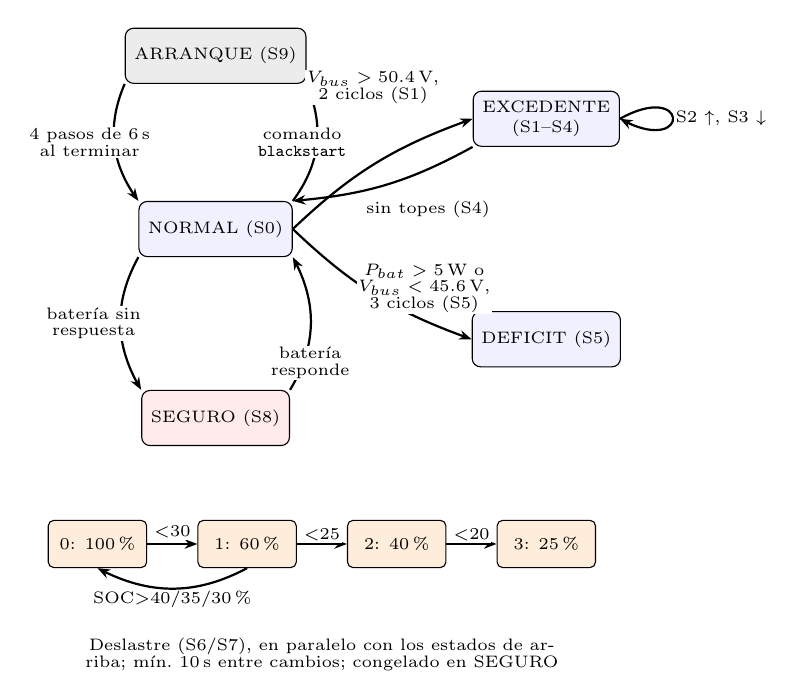
\begin{tikzpicture}[font=\fontsize{6.5}{7}\selectfont,
  st/.style={draw,rounded corners=3pt,minimum width=1.75cm,minimum height=.7cm,align=center,fill=blue!6},
  sh/.style={draw,rounded corners=2pt,minimum width=1.25cm,minimum height=.6cm,align=center,fill=orange!14},
  tr/.style={-{Stealth[length=1.6mm]},thick},
  lb/.style={font=\fontsize{5.6}{6}\selectfont,align=center,fill=white,inner sep=.6pt}]
\node[st,fill=gray!15] (a) at (1.9,2.9) {ARRANQUE (S9)};
\node[st] (n) at (1.9,0.7) {NORMAL (S0)};
\node[st,fill=red!8] (s) at (1.9,-1.7) {SEGURO (S8)};
\node[st] (e) at (6.1,2.1) {EXCEDENTE\\(S1--S4)};
\node[st] (d) at (6.1,-0.7) {DEFICIT (S5)};
\draw[tr] (a.south west) to[bend right=30] (n.north west);
\draw[tr] (n.north east) to[bend right=30] (a.south east);
\node[lb] at (0.3,1.8) {4 pasos de 6\,s\\al terminar};
\node[lb] at (3.0,1.8) {comando\\\texttt{blackstart}};
\draw[tr] (n.east) to[bend left=12] (e.west);
\draw[tr] (e.south west) to[bend left=12] (n.north east);
\node[lb] at (3.9,2.5) {$V_{bus}>50.4$\,V,\\2 ciclos (S1)};
\node[lb] at (4.6,0.95) {sin topes (S4)};
\draw[tr] (n.east) to[bend right=12] (d.west);
\node[lb] at (4.55,-0.05) {$P_{bat}>5$\,W o\\$V_{bus}<45.6$\,V,\\3 ciclos (S5)};
\draw[tr] (n.south west) to[bend right=30] (s.north west);
\draw[tr] (s.north east) to[bend right=30] (n.south east);
\node[lb] at (0.35,-0.5) {batería sin\\respuesta};
\node[lb] at (3.1,-1.0) {batería\\responde};
\draw[tr] (e.east) .. controls +(.9,.5) and +(.9,-.5) .. node[lb,right]{S2 $\uparrow$, S3 $\downarrow$} (e.east);
\node[sh] (h0) at (0.4,-3.3) {0: 100\,\%};
\node[sh] (h1) at (2.3,-3.3) {1: 60\,\%};
\node[sh] (h2) at (4.2,-3.3) {2: 40\,\%};
\node[sh] (h3) at (6.1,-3.3) {3: 25\,\%};
\draw[tr] (h0) -- node[lb,above=1pt]{$<$30} (h1);
\draw[tr] (h1) -- node[lb,above]{$<$25} (h2);
\draw[tr] (h2) -- node[lb,above]{$<$20} (h3);
\draw[tr] (h1.south) to[bend left=28] node[lb,below]{SOC$>$40/35/30\,\%} (h0.south);
\node[lb,fill=none,text width=6.2cm,align=center] at (3.25,-4.7) {Deslastre (S6/S7), en paralelo con los estados de arriba; mín.\ 10\,s entre cambios; congelado en SEGURO};
\end{tikzpicture}
\caption{Diagrama de estados del SCADA y, abajo, su deslastre escalonado.}
\label{fig:estados}
\end{figure}

\textbf{Excedente (S1--S4).} Si el bus supera 50.4\,V durante dos ciclos, S1 entra a EXCEDENTE y fija un tope absoluto a los generadores (primero la PV, hasta un piso de 15\,W, y luego la eólica, con piso de 13.4\,W). El escalón de recorte de S2 es proporcional al exceso de tensión,
\begin{equation}
\label{eq:dP}
\Delta P=\min\{30,\,5+10\,(V_{bus}-50.4)\}\ \text{W},
\end{equation}
y se aplica cada 6\,s, o cada 2\,s si el bus supera 53\,V; en sem.~13 era fijo (5\,W). S3 suelta un escalón cuando la batería vuelve a descargar y S4 devuelve los generadores a MPPT.

\textbf{Déficit y deslastre (S5--S7).} En sem.~13 el deslastre tenía un solo nivel (carga al 60\,\% con SOC $<20$\,\%) y no evitó que el SOC bajara a 13.0\,\%. Ahora es escalonado y anticipado: la carga se lleva al 60, 40 y 25\,\% de su perfil cuando el SOC baja de 30, 25 y 20\,\%, y se restaura un nivel cada vez que supera 40, 35 y 30\,\% (histéresis de 10 puntos), con un tiempo mínimo de 10\,s entre cambios.

\textbf{Justificación de los umbrales.} Con la aceleración de $60\times$ (ec.~\ref{eq:SOC}), el SOC cae 0.12, 0.23 y 0.80\,\%/s con 1, 2 y 7\,A (descarga máxima). Con un déficit típico de 1--2\,A, 5 puntos entre niveles son 22--43\,s y los 10 de histéresis 43--87\,s, mucho más que el ciclo de 1\,s y el mínimo de 10\,s, así que el SCADA no oscila; con 7\,A esos 5 puntos se cruzarían en 6\,s, por lo que el mínimo no puede ser mayor. El nivel 1 se fija 10 puntos sobre el 20\,\% de reserva como margen de reacción.

\textbf{Arranque en negro (S9).} Por comando, cuatro pasos de 6\,s: todo en modo seguro (bus caído emulado), la batería forma el bus, la PV y la eólica reconectan en MPPT y por último se reconecta la carga.

\subsection{Qué es hardware y qué es emulación}

La Tabla~\ref{tab:hw} separa lo que es físico de lo que es modelo. \emph{Todo lo que ocurre entre una fuente y el bus es software}: no hay etapa de potencia, y por eso este trabajo valida la supervisión y el control, no la transferencia de potencia.

\begin{table}[!t]
\caption{Hardware real frente a emulación}
\label{tab:hw}
\centering
\scriptsize\setlength{\tabcolsep}{3pt}
\begin{tabular}{|p{1.45cm}|p{2.7cm}|p{2.6cm}|}
\hline
 & \textbf{Hardware real} & \textbf{Emulado (firmware)} \\
\hline
Cómputo y comunicación & 4 STM32F303K8, ESP32-S3, bus I2C a 100\,kHz, Wi-Fi/MQTT, PC con registrador y tablero & --- \\ \hline
Fuentes & --- & Irradiancia, viento, perfiles de carga, reloj de 360\,s \\ \hline
Potencia & --- & Convertidores promediados, batería (Thevenin, SOC $\times60$), bus de 48\,V \\ \hline
Perturbaciones & Desenergizar la placa del PV (E6) & Apagón de E5 (modo seguro); no hay contactor de aislamiento \\ \hline
\end{tabular}
\end{table}

\section{Metodología y Criterios de Aceptación}
\label{sec:metodo}

Las pruebas se hicieron con el sistema integrado y el SCADA activo; el registrador guarda cada mensaje MQTT crudo y todas las métricas salen de ese CSV. Cada experimento es una captura continua con los cuatro STM reiniciados a la vez. P0, E1, E2, E5 y E6 usaron el firmware v7; E3 y E4 se repitieron con el gateway \texttt{v7+diag}, de lógica idéntica, que solo agrega la medición de latencias. La semana 13 (firmware v6) es solo la línea base. Se descartaron dos corridas con el SCADA pausado por error y dos con la carga limitada al 40\,\%.

Los criterios (Tabla~\ref{tab:crit}) son propuestas del equipo, fijadas antes de medir; ninguno proviene de una norma de tensión y la última columna dice de dónde sale cada número.

\begin{table}[!t]
\caption{Experimentos, criterios de aceptación y su justificación}
\label{tab:crit}
\centering
\scriptsize\setlength{\tabcolsep}{2pt}
\begin{tabular}{|c|p{1.95cm}|p{2.75cm}|}
\hline
\textbf{Exp.} & \textbf{Criterio} & \textbf{Justificación} \\
\hline
P0 & 0 de 3 amaneceres con el PV atascado & En sem.~13 fallaron 3 de 3 \\ \hline
E1 & $V_{bus}$ en banda $\ge95$\,\%; SOC mín. $\ge20$\,\% & Banda ±5\,\% de diseño con 5\,\% de holgura; 20\,\% es la reserva mínima del Li-ion y el límite del nivel 3 \\ \hline
E2 /E3 & $V_{bus,max}\le53$\,V; SCADA reduce $\ge30$\,\% el tiempo $>53$\,V; $\le2$ entradas a S1 (E3) & 53\,V es $\approx+10$\,\% y el umbral de recorte rápido de S2; 30\,\% es la mejora mínima que el equipo consideró material; $\approx$1 entrada por día simulado \\ \hline
E4 & Deslastre $\le2$\,s tras el umbral; SOC mín. $\ge20$\,\% & 2 ciclos de 1\,s del SCADA; mismo SOC mínimo \\ \hline
E5 & Duración $\le30$\,s; $V_{bus}$ en ±10\,\% & 4 pasos $\times$ 6\,s $=24$\,s más 25\,\% de margen; ±10\,\% (43.2--52.8\,V) admite el transitorio de la secuencia \\ \hline
E6 & Detección $\le5$\,s; $V_{bus}$ en banda; recuperación & 3 sondeos fallidos a 1\,Hz $\approx3$\,s más margen \\ \hline
\end{tabular}
\end{table}

\section{Resultados}

Las figuras de resultados marcan los umbrales de la Tabla~\ref{tab:crit}: banda de ±5\,\% (45.6 y 50.4\,V), 53\,V, y los umbrales de deslastre del SOC (30 y 25\,\%) y su mínimo aceptable (20\,\%).

\subsection{P0: PV corregido y deslastre escalonado}
\label{sec:p0}

Se registró el sistema 1194\,s ($\approx$3.3 días simulados) con la carga alternando entre residencial e industrial (Fig.~\ref{fig:p0}). El PV arrancó solo en los tres amaneceres ($t\approx350$, 711 y 1072\,s) y alcanzó el 10\,\% de su pico en 2.8, 3.4 y 4.9\,s, con la referencia de tensión entre 15.8 y 19.4\,V, lejos del límite de 23.8\,V que causaba el fallo. El SOC mínimo fue 24.5\,\%; el nivel 1 se activó con el SOC en 29.8--29.9\,\%, el nivel 2 en 24.9\,\% y la restauración llegó con 40.3, 40.1 y 35.1\,\%, como indica el diseño. El bus estuvo en 48.00\,V todo el tiempo. La generación fue 90--96\,\% del consumo: el deslastre evita agotar la batería, pero no corrige un dimensionamiento justo.

\begin{figure}[!t]
\centering
\includegraphics[width=\columnwidth]{P0.png}
\caption{P0: potencia del PV, SOC con los eventos de deslastre (S6) y restauración (S7), y $V_{bus}$. Líneas punteadas verticales: amaneceres simulados.}
\label{fig:p0}
\end{figure}






\subsection{E1: operación nominal con carga alternante}

Con la carga alternando cada 120\,s durante 1047\,s, el bus estuvo en banda el 100\,\% del tiempo (48.00\,V) y el SOC cayó de 45.0\,\% a un mínimo de \textbf{24.8\,\%} (16.8\,\% en sem.~13). La batería descargó el 63.1\,\% del tiempo: con carga residencial la generación media (73.3\,W) supera a la carga (55.3\,W) y con la industrial ocurre lo contrario (75.4 contra 101.0\,W). El deslastre actuó en el nivel 1 a los 574\,s (SOC 29.9\,\%) y en el nivel 2 a los 726\,s (24.9\,\%), y se restauró a los 785 y 803\,s, cada evento en la misma muestra del cruce ($\le1$\,s). No hubo EXCEDENTE: E1 valida las reglas de déficit, no las de excedente.

\subsection{E2 y E3: excedente, sin y con SCADA}

\textbf{E2, excedente con SCADA.} Con la carga reducida a 40\,\%, la batería llegó a $\approx$98\,\% hacia $t=400$\,s y dejó de absorber potencia; el sobrante elevó el bus sobre 50.4\,V y S1 entró en 404.7\,s (Fig.~\ref{fig:e2}). Hubo tres episodios (S1 a S4: 404.7--689.7, 737.8--1030.8 y 1112.7--1372.8\,s) con $V_{bus}$ máximo de 57.29, 57.90 y 57.82\,V; en total 313\,s fuera de banda (22.0\,\% de 1428\,s), 263\,s sobre 53\,V y recorte de hasta 87\,W. De los 139 escalones S2, 128 fueron de $+0$\,W: el recorte ya estaba en su piso. Frente a sem.~13 (9.2\,\% fuera de banda) es peor, y no lo atribuimos al SCADA sin una corrida de E2 sin SCADA de igual perfil.

\begin{figure}[!t]
\centering
\includegraphics[width=\columnwidth]{E2_serie.png}
\caption{E2: $V_{bus}$ (con la línea de 53\,V), potencias y recorte. Sombreado: EXCEDENTE.}
\label{fig:e2}
\end{figure}


\textbf{E3, sin y con SCADA, en fase.} Se repitió E3 con el gateway \texttt{v7+diag}: A (sin SCADA, 986\,s) y B (con SCADA, 1005\,s), con el mismo procedimiento (carga al 40\,\% hasta $t\approx290$\,s y luego residencial) y los cuatro STM energizados con un solo interruptor (Fig.~\ref{fig:e3}, Tabla~\ref{tab:e3r}). \emph{No quedaron perfectamente en fase}: los amaneceres difieren 4.1\,s. El criterio de fase se había fijado en $\le2$\,s antes de medir y se \emph{relajó a $\le5$\,s después de la repetición}, porque cada STM32 inicia su reloj de día al reiniciarse y el arranque simultáneo de las cuatro placas no se logró con mejor precisión; 5\,s son 1.4\,\% del día de 360\,s y no cambian la forma de las curvas. Con el criterio relajado se cumple; con el original no. El SOC en $t=302$\,s difiere 0.4 puntos (cumple $\le2$) y A dura 14\,s menos que el mínimo de 1000\,s. Antes del recorte, la curva de PV de B coincide con la de A (0.2\,W RMS) al desplazarla 4.5\,s, y la carga al desplazarla 2\,s; el desfase parece del registrador y de la STM del PV. Se compara la ventana común $t\in[302,985]$\,s.

\begin{table}[!t]
\caption{E3 (retoma): sin SCADA (A) y con SCADA (B), ventana común 302--985\,s}
\label{tab:e3r}
\centering
\scriptsize
\begin{tabular}{|l|c|c|}
\hline
\textbf{Métrica} & \textbf{A (sin SCADA)} & \textbf{B (con SCADA)} \\
\hline
Tiempo con $V_{bus}>53$\,V & 507\,s (74.2\,\%) & 175\,s (25.6\,\%) \\ \hline
Tiempo fuera de banda & 512\,s (75.0\,\%) & 202\,s (29.6\,\%) \\ \hline
$>53$\,V, corrida completa & 509\,s (51.6\,\%) & 176\,s (17.5\,\%) \\ \hline
$V_{bus}$ máximo (V) & 58.00 & 57.87 \\ \hline
Recorte máx.\ (W) / entradas a S1 & 0 / --- & 77 / 2 \\ \hline
S1 tras la 1.ª muestra $>50.4$\,V & --- & $\approx$1\,s \\ \hline
Amanecer del PV (s) & 350.0 & 345.9 \\ \hline
SOC en $t=302$\,s (\%) & 95.7 & 95.3 \\ \hline
\end{tabular}
\end{table}

\begin{figure}[!t]
\centering
\includegraphics[width=\columnwidth]{E3_AB.png}
\caption{E3 (retoma): $V_{bus}$ sin SCADA (A) y con SCADA (B), y SOC. La línea de trazo y punto marca $t=302$\,s; las punteadas, los amaneceres.}
\label{fig:e3}
\end{figure}

\begin{figure}[!t]
\centering
\includegraphics[width=\columnwidth]{E4_serie.png}
\caption{E4 (retoma): $V_{bus}$, potencias y SOC con los eventos de deslastre (S6) y restauración (S7), con carga industrial fija.}
\label{fig:e4}
\end{figure}


El SCADA redujo de 74.2 a 25.6\,\% el tiempo sobre 53\,V en la ventana común ($-65.5\,\%$; $-66.1\,\%$ en la corrida completa) y entró a S1 $\approx$1\,s después de la primera muestra sobre 50.4\,V, con solo 2 entradas. El par de la primera tanda (A de 1003\,s y B de 1076\,s, con $\approx$18\,s de desfase) dio 52.5 contra 15.2\,\% ($-71\,\%$), de modo que la reducción se reprodujo en dos pares (65--71\,\%). No se evitó el pico: el bus llegó a 57.87\,V, como sin SCADA, con la batería llena ($\mathrm{SOC}\ge99.8\,\%$) y el recorte en su piso (13--15\,W por generador), que supera la carga de 16--32\,W; ahí el SCADA repite escalones de $+0$\,W sin poder bajar más.

\subsection{E4: déficit industrial con deslastre escalonado}

Con carga industrial fija (\texttt{load ind} a $t=36.6$\,s), SOC inicial de 47.1\,\% y el SCADA activo, el deslastre se activó cuatro veces (Fig.~\ref{fig:e4}). Se completaron \textbf{tres ciclos} de deslastre a restauración total (334--477\,s, 561--853\,s y 935--1197\,s, de 143, 292 y 262\,s); un cuarto empezó a los 1287\,s (nivel 2 a los 1439\,s) y seguía abierto al cerrar a 1467\,s, con el SOC en 25.2\,\% y subiendo. Los niveles se activaron con el SOC en 29.8--29.9\,\% y 24.9\,\% y se restauraron con 35.1 y 40.1--40.2\,\%, cada uno en la misma muestra del cruce ($\le1$\,s). El \textbf{SOC mínimo fue 24.4\,\%} ($t=1447$\,s), por lo que el nivel 3 nunca actuó (13.0\,\% en sem.~13). El bus estuvo en 48.00\,V todo el tiempo, con 660\,s en DEFICIT (45\,\%) y 878\,s (60\,\%) con deslastre activo. Una corrida anterior terminó con el SOC en 21.4\,\% y el tercer ciclo abierto; esta lo cierra y la reemplaza.


\subsection{E5: arranque en negro}

La secuencia de cuatro pasos duró 24.0\,s de día ($t=96.6$\,s) y 24.0\,s de noche ($t=326.5$\,s) (24.8 y 25.4\,s en sem.~13), sin subsistemas fuera de línea (Fig.~\ref{fig:e5}). De noche el bus se quedó en 48.00\,V. De día subió a 53.81\,V ($+12.1\,\%$) durante 4.0\,s: la carga baja a $\approx$10\,W, el PV sigue entregando $\approx$140\,W y la batería forma el bus con la corriente limitada en modo seguro. Supera por 1.0\,V el límite de $\pm10$\,\% (52.8\,V) y es peor que en sem.~13 (52.92\,V). El apagón es emulado: E5 valida la reconexión, no un arranque desde un bus desenergizado.

\begin{figure}[!t]
\centering
\includegraphics[width=\columnwidth]{E5_blackstart.png}
\caption{E5: arranque en negro de día y de noche. Sombreado: secuencia de 4 pasos; línea roja: límite de $+10$\,\%.}
\label{fig:e5}
\end{figure}



\begin{figure}[!t]
\centering
\includegraphics[width=\columnwidth]{E6_falla_PV.png}
\caption{E6: falla emulada del PV (zona sombreada) con las marcas de fuera de línea y en línea.}
\label{fig:e6}
\end{figure}


\subsection{E6: falla de un generador (emulada)}

No hay contactor físico ni modo desconectado en el firmware, y no se modificó: la falla se emuló desconectando el USB de la placa del PV $\approx$44\,s, con el SCADA activo (Fig.~\ref{fig:e6}). La última lectura del PV fue en $t=35.98$\,s (71.7\,W) y el gateway lo marcó fuera de línea en $t=39.03$\,s: \textbf{detección en 3.0\,s}, igual a 3 sondeos fallidos de 1\,s. La generación bajó de $\approx$109 a 15--20\,W (queda la eólica), la batería pasó de cargar $\approx$83\,W a cubrir el faltante y $V_{bus}$ se mantuvo en 48.00\,V: \textbf{recuperación del bus en 0\,s}. El PV volvió a línea en $t=79.97$\,s y arrancó en MPPT sin bloquearse; recuperó el 50, 90 y 100\,\% de su potencia previa a los 23, 45 y 53\,s, tiempo que sigue la rampa de irradiancia (su placa reinicia el día simulado) y no mide al MPPT.

\subsection{Latencias I2C y MQTT}

El gateway \texttt{v7+diag} mide cada segundo el tiempo de cada transacción I2C, el de la publicación MQTT y un eco ESP32--broker--ESP32. La Tabla~\ref{tab:lat} reúne 3461 ciclos de E3 (A y B) y E4, con el broker en el PC y el Wi-Fi de un teléfono como punto de acceso.

\begin{table}[!t]
\caption{Latencias medidas (3461 ciclos de 1\,s, 3 corridas)}
\label{tab:lat}
\centering
\scriptsize\setlength{\tabcolsep}{3pt}
\begin{tabular}{|l|c|c|c|c|}
\hline
\textbf{Medida} & \textbf{Mediana} & \textbf{p95} & \textbf{p99} & \textbf{Máx.} \\ \hline
Transacción I2C, promedio por ciclo (ms) & 1.94 & 1.95 & 1.96 & 1.96 \\ \hline
Transacción I2C más lenta del ciclo (ms) & 2.95 & 2.98 & 3.04 & 3.08 \\ \hline
Publicación MQTT (ms) & 0.49 & 0.62 & 1.26 & 1.67 \\ \hline
Eco MQTT, ida y vuelta (ms) & 54 & 159 & 248 & 513 \\ \hline
Periodo del mensaje de estado (s) & 1.000 (media) & --- & 1.21 & 2.66 \\ \hline
\end{tabular}
\end{table}

Cada ciclo hace 8 transacciones I2C ($\approx$15.5\,ms, 1.6\,\% del periodo) sin reintentos por lecturas corruptas. El SCADA no depende de MQTT: corre en el ESP32 con datos leídos por I2C, y el eco solo afecta al registrador y al tablero. Con sondeo de 1\,s, el dato que ve el SCADA tiene a lo sumo un ciclo más $\approx$3\,ms de edad, lo que explica que S1 entre $\approx$1\,s después del primer dato sobre 50.4\,V y que la detección de una falla tarde 3\,s. El eco tiene una cola larga (2.5\,\% sobre 200\,ms, 0.06\,\% sobre 500\,ms, máximo 0.51\,s) atribuible al Wi-Fi del teléfono; no se midió la latencia de un comando del PC a la STM.

\subsection{Resumen frente a los criterios}
\label{sec:resumen}

\begin{table}[!t]
\caption{Resultados frente a los criterios de aceptación}
\label{tab:res}
\centering
\scriptsize\setlength{\tabcolsep}{2.5pt}
\begin{tabular}{|c|p{3.9cm}|c|}
\hline
\textbf{Exp.} & \textbf{Resultado medido} & \textbf{Estado} \\
\hline
P0 & 0 de 3 amaneceres atascados & \ding{51} \\ \hline
E1 & Banda 100\,\%; SOC mín. 24.8\,\% & \ding{51}\,/\,\ding{51} \\ \hline
E2/E3 & $V_{bus,max}$ 57.87\,V; reducción $>53$\,V de 66 y 71\,\% (dos pares); 2 entradas a S1 & \ding{55}\,/\,\ding{51}\,/\,\ding{51} \\ \hline
E3 fase & Amanecer 4.1\,s; SOC 0.4 pts; A de 986\,s & \ding{55}\,/\,\ding{51}\,/\,\ding{55} \\ \hline
E4 & Deslastre $\le1$\,s; SOC mín. 24.4\,\%; tres ciclos completos & \ding{51}\,/\,\ding{51} \\ \hline
E5 & 24.0 / 24.0\,s; $+12.1\,\%$ de día, 0\,\% de noche & \ding{51}\,/\,\ding{55} (día) \\ \hline
E6 & Detección 3.0\,s; $V_{bus}$ 48.00\,V; PV recuperado (emulado) & \ding{51} \\ \hline
\end{tabular}
\end{table}

Estos son los resultados más recientes y reemplazan a los de la semana 13: mejoran el SOC mínimo (E1: 16.8 a 24.8\,\%; E4: 13.0 a 24.4\,\%), la reducción del tiempo sobre 53\,V ($-27$ a $-66$/$-71\,\%$) y el arranque en negro (24.8 y 25.4 a 24.0\,s). No se cumplen $V_{bus}\le53$\,V (57.87\,V), los ±10\,\% del arranque en negro de día (53.81\,V) ni la fase de E3.

\section{Alineación con ISA-101 e ISA-18.2}
\label{sec:isa}

El tablero es un demostrador para público no técnico, no una interfaz de operación; aun así se evaluó frente a las dos normas, que aquí son referencia y no un requisito certificado. ISA-101~\cite{isa101} recomienda organizar las pantallas en una jerarquía de niveles, reservar el color para las condiciones anormales y mostrar cada valor frente a lo que es normal. ISA-18.2~\cite{isa182} define el ciclo de vida de las alarmas (filosofía, identificación, racionalización, monitoreo) y toma de EEMUA~191~\cite{eemua191} los valores de referencia: de 1 a 2 alarmas por 10\,min es manejable y más de 10 en 10\,min es una \emph{inundación}.

\textbf{HMI (ISA-101).} El tablero sigue la jerarquía (nivel 1: mapa de energía; nivel 2: gráficas y cifras; nivel 3: las cuatro partes; y una pestaña de control) y sigue en parte el valor en contexto (mensaje de estado y bandas de 45.6 y 50.4\,V en las gráficas). No sigue la recomendación del color, porque usa un color fijo por fuente (azul, amarillo, verde, rosa) sobre fondo oscuro cuando ISA-101 sugiere reservarlo para lo anormal sobre fondos neutros, ni la de alarmas, porque lista eventos con la regla S$n$ sin prioridad ni reconocimiento. Es una revisión del tablero, no una prueba con operadores, y el texto de ISA-101 se consultó a través de fuentes secundarias.

\textbf{Alarmas (ISA-18.2).} Se racionalizaron las condiciones del SCADA (Tabla~\ref{tab:isa182}): solo las que exigen una respuesta del operador son alarmas; los ajustes automáticos y los retornos son eventos que se registran. Es una propuesta; el tablero actual no la implementa y las cifras se recalcularon sobre el registro de eventos. El repositorio incluye una capa de alarmas del PC (\texttt{scada\_pc/alarmas.py}) con prioridad, retardos y banda muerta, aún no integrada al tablero.

\begin{table}[!t]
\caption{Racionalización propuesta de las condiciones del SCADA}
\label{tab:isa182}
\centering
\scriptsize\setlength{\tabcolsep}{2.5pt}
\begin{tabular}{|p{2.5cm}|p{1.45cm}|c|p{0.95cm}|}
\hline
\textbf{Condición} & \textbf{Consecuencia} & \textbf{Prior.} & \textbf{Trato} \\ \hline
S8: batería sin respuesta & Bus sin regular & Alta & Alarma \\ \hline
S1: entrada a EXCEDENTE & Hasta 58\,V & Alta & Alarma \\ \hline
Generador sin respuesta & Pierde generación & Media & Alarma \\ \hline
S6: deslastre (nivel 3) & Carga no servida & Media (alta) & Alarma \\ \hline
S5: DEFICIT & Batería cubre & Baja & Estado \\ \hline
S2, S3, S4, S7, S9 & Ajuste o retorno & --- & Evento \\ \hline
\end{tabular}
\end{table}

Tal como está, el tablero anuncia todo como evento: en E3~B hay 114 eventos del SCADA (S1--S7) en 1005\,s ($\approx$68 por 10\,min, y hasta 31 en un minuto) y en E2 174 en 1428\,s ($\approx$73 por 10\,min), una inundación según la definición anterior. La causa es que S2 se repite cada $\approx$2\,s con $+0$\,W con el bus sobre 53\,V y el recorte en su piso: 85 de 92 escalones en E3~B y 128 de 139 en E2 (92\,\% en ambos), una alarma \emph{chattering}. Con la clasificación de la Tabla~\ref{tab:isa182} (S1, S6 y S8 como alarmas) la tasa baja a 1.2 por 10\,min en E3~B, 1.3 en E2, 1.1 en E1 y 2.9 en E4, donde la carga industrial sostenida provoca 7 subidas de nivel en 24\,min. Solo E4 supera el valor de 1 a 2 por 10\,min, en una prueba pensada para llevar el SOC al límite. Suprimir los escalones de $+0$\,W requiere cambiar el firmware, lo que no se hizo.

\section{Comparación con las Arquitecturas de Referencia}

Es una emulación de señal y control, no una réplica de los bancos físicos de los demás subgrupos: el PV equivale al modelo simplificado de~\cite{aristizabal2026pv}, la turbina simplifica la regulación del bus que el banco real~\cite{gonzalez2026eolica} no logra sin etapa activa, y la batería es lo más alineado con~\cite{vega2026bateria}. La brecha mayor es la electrónica de potencia~\cite{pinto2026peb}, y el SCADA cambia el PLC con Modbus TCP de~\cite{alvarez2026scada} por un gateway ESP32 con MQTT, más liviano y no equivalente (Anexo~H).

\section{Conclusiones}

Se construyó una microrred DC de 48\,V emulada en la que cuatro subsistemas con modelo, convertidor y control local comparten un reloj y un SCADA los acopla y supervisa. Frente a la semana 13: (i) el PV arranca en 3 de 3 amaneceres, (ii) el bus se mantiene en 48.00\,V mientras la batería lo regula, incluso al perder un generador (detección en 3.0\,s), (iii) el deslastre sube el SOC mínimo de 13.0 a 24.4\,\% con carga industrial (tres ciclos completos) y de 16.8 a 24.8\,\% con carga alternante, y (iv) el SCADA reduce 66--71\,\% el tiempo sobre 53\,V en dos pares de corridas. No se cumple el tope de 53\,V (pico de $\approx$58\,V con la batería llena y el recorte en su piso), ni los $\pm10$\,\% del arranque en negro de día (53.81\,V); la fase de E3 (4.1\,s) cumple solo con el criterio relajado a $\le5$\,s, y en E2 el bus pasó más tiempo fuera de banda que en sem.~13 (22.0 frente a 9.2\,\%). Las latencias son bajas frente al periodo de 1\,s, y la mayor brecha frente a las normas es el registro de eventos, que se vuelve una inundación por escalones repetidos de $+0$\,W.

\textbf{Trabajo futuro.} Pasar la microrred a físico: montar todos los subsistemas, convertidores y el SCADA en hardware real.

Código, datos y anexos técnicos (modelos, convertidor, bus I2C, lazos, reglas del SCADA y comparación): \href{https://github.com/soofffp/VITA-DC-Microgrid}{\texttt{github.com/soofffp/VITA-DC-Microgrid}}. Se usó un modelo de lenguaje~\cite{anthropic2026claude} para revisar formato, citas, gramática y el análisis de los registros; los datos y las conclusiones son de los autores.

\begin{thebibliography}{00}

\bibitem{aristizabal2026pv}
L. Á. Aristizábal Correa, J. F. Angulo Rubiano, and S. J. Fonseca Boada, ``Emulación de Arreglos Fotovoltaicos para Microrredes DC de Laboratorio: Pipeline en Python, Comparación de Modelos Eléctricos e Integración SCPI--Modbus TCP,'' Informe técnico, Departamento de Ingeniería Eléctrica y Electrónica, Universidad de los Andes, Bogotá, Colombia, 2026.

\bibitem{gonzalez2026eolica}
J. D. González Cubides, J. D. Roa Ballén, and C. D. González Mayorga, ``Emulación experimental y supervisión SCADA de un subsistema eólico de 300 W para microrredes DC basado en PMSG,'' Informe técnico, Departamento de Ingeniería Eléctrica y Electrónica, Universidad de los Andes, Bogotá, Colombia, 2026.

\bibitem{vega2026bateria}
L. D. Vega Moreno, J. S. Torres Soler, and J. J. Carrera Luna, ``Integración y caracterización de un sistema de almacenamiento 10s5p basado en Ion-Litio para microrredes DC,'' Departamento de Ingeniería Eléctrica y Electrónica, Universidad de los Andes, Bogotá, Colombia, 2026.

\bibitem{hernandez2026carga}
J. F. Hernández, D. E. Niño Jimenez, and J. J. Castillo Urbano, ``Metodología de Emulación de Perfiles de Demanda en Microrredes DC mediante Integración C-HIL y Cargas Programables,'' Informe técnico, Departamento de Ingeniería Eléctrica y Electrónica, Universidad de los Andes, Bogotá, Colombia, 2026.

\bibitem{isa101}
ANSI/ISA-101.01-2015, \emph{Human Machine Interfaces for Process Automation Systems}, International Society of Automation, Research Triangle Park, NC, USA, 2015.

\bibitem{isa182}
ANSI/ISA-18.2-2009, \emph{Management of Alarm Systems for the Process Industries}, International Society of Automation, Research Triangle Park, NC, USA, 2009.

\bibitem{eemua191}
EEMUA Publication 191, \emph{Alarm Systems: A Guide to Design, Management and Procurement}, 3rd ed., Engineering Equipment and Materials Users' Association, London, U.K., 2013.

\bibitem{pinto2026peb}
J. D. Pinto Cardenas and J. J. Vasquez Polaina, ``Informe final: Bloque Modular de Electrónica de Potencia (PEBB) basado en un Convertidor DC--DC en Configuración de Medio Puente con IGBT para Microrredes DC,'' Departamento de Ingeniería Eléctrica y Electrónica, Universidad de los Andes, Bogotá, Colombia, 2026.

\bibitem{alvarez2026scada}
M. Alvarez Valenzuela, A. F. Mosquera Gómez, and Ó. M. Cristancho Florez, ``Informe Final: SCADA,'' Taller de Potencia, Departamento de Ingeniería Eléctrica y Electrónica, Universidad de los Andes, Bogotá, Colombia, 2026.

\bibitem{anthropic2026claude}
Anthropic, ``Claude (Sonnet),'' modelo de lenguaje de gran escala utilizado para la revisión de formato del documento, verificación de consistencia de citas, y revisión de gramática y ortografía, Anthropic, 2026. [En línea]. Disponible: https://www.anthropic.com/claude

\end{thebibliography}

\end{document}
